\documentclass[11pt,a4paper]{article}
\usepackage[margin=2.5cm]{geometry}
\usepackage{graphicx}
\title{Labwork 9: Histogram Equalization}
\author{Duong Tan Binh \\ Student ID: 2540007}
\date{}
\begin{document}
\maketitle
\section{Histogram}
I use the grayscale image from Lab 4. Each thread reads one row and
counts its gray levels in a separate 256-bin histogram.
A second kernel adds the row histograms, with one thread per bin.
Different threads never update the same row histogram, so atomic
operations are not needed.

\section{Equalization}
I add the histogram counts in order on the CPU, as shown in the slide.
For each level, I set its new value to \texttt{255 * cumulative / pixelCount},
keeping the integer part. This follows the CDF formula in the slide.
The GPU then looks up the new value for every pixel.

\section{Results}
\begin{verbatim}
Pixels: 307200
Histogram total: 307200
Input range: 0 255
Output range: 0 255
\end{verbatim}
I checked the histogram and the output image with NumPy and they are the same.
The output histogram is more spread out, but it is not exactly flat.

\begin{center}
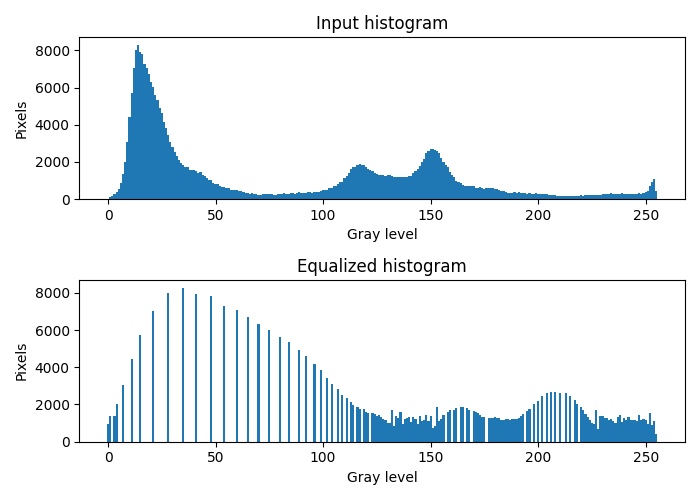
\includegraphics[width=0.48\textwidth]{histograms.png}
\end{center}
\begin{center}
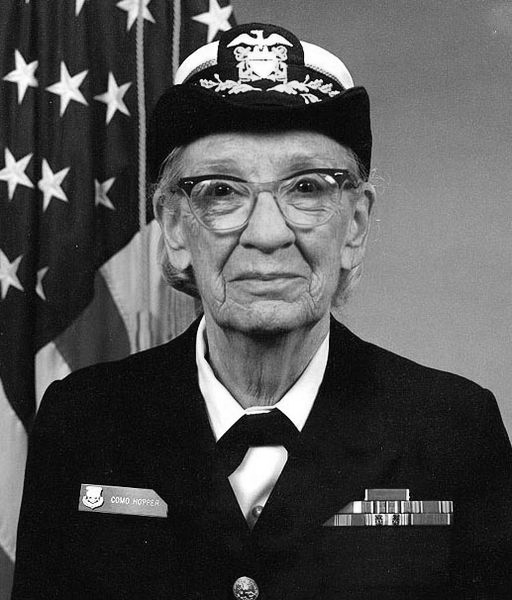
\includegraphics[width=0.18\textwidth]{input.png}
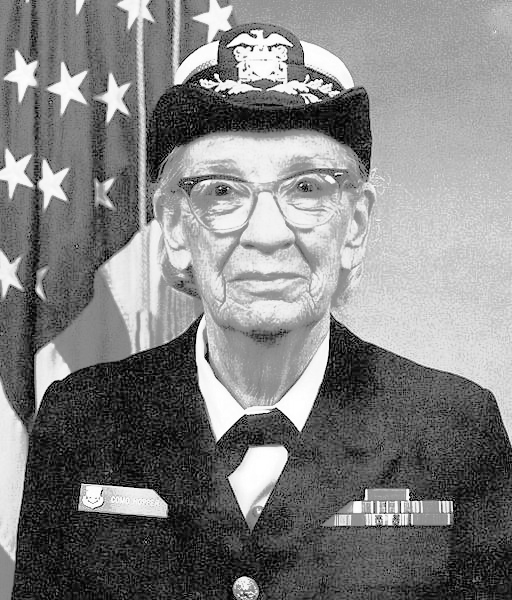
\includegraphics[width=0.18\textwidth]{equalized.png}
\end{center}
Input grayscale image and equalized result.

\end{document}
